\documentclass[10pt,a4paper]{report}
\usepackage[utf8]{inputenc}
\usepackage{amsmath,wasysym}
\usepackage{amsfonts}
\usepackage{amssymb}
\usepackage{amsthm}
\usepackage{bbm}
\usepackage{dsfont}
\usepackage{graphicx}
\usepackage{picins}
\usepackage[section]{placeins}
\usepackage{ngerman}
\usepackage{geometry}
\usepackage{enumitem}
\usepackage{extarrows}
\usepackage{setspace}
\usepackage{float}
\usepackage{mathrsfs} 
\usepackage{subfigure}
\usepackage{csquotes}
\usepackage{ulem}


\title{Modellierung 1, Praktikum, 17.07.2017 bis 28.07.2017}
%\subtitle{}
\author{Christian Ali, Janka Bauer, Niklas Bockius}
\date{28.07.2017}

\begin{document}

\textit{\large Modellierung 1, Praktikum, 17.07.2017 bis 28.07.2017}

\textit{Gruppe Deep Learning}

\textit{Christian Ali, Janka Bauer, Niklas Bockius}

\bigskip
\bigskip
\uline{Montag, 17.07.17:}
\begin{itemize}
	\item Vorbesprechung und Einführung in Deep Learning 
	\item Initialisierung eines Git-Repository 
	\item Einarbeiten
\end{itemize}

\bigskip	
\uline{Dienstag, 18.07.17:}
\begin{itemize}
\item AutoEncoder für MNIST aufbauend auf dem Tutorial: erste Hälfte (bis Bottleneck) aus Tutorial übernommen, zweite Hälfte selbst erstellt (alles reverse)\\
am Ende des Tages unschöne Ergebnisse:
	\begin{itemize}
	\item erst regelmäßiges Rauschen 
	\item dann Zahl sehr verpixelt, aber erkennbar 
	\end{itemize}
\item Verbesserungen durch:
	\begin{itemize}
	\item loss-Funktion mit least squares statt mit cross-entropy berechnet
	\item Anzahl der Channels (auf dem Rückweg) erhöht
	\end{itemize}  	                        
\end{itemize}

\begin{figure}[H]
\centering
\subfigure[pic1, Original]{
\includegraphics[scale=2.5]{mnist_orig1_badLoss.png}} 
\hspace{0.5cm}
\subfigure[pic1, generiert mit cross-entropy und einem Channel]{
\includegraphics[scale=2.5]{mnist_gen1_badLoss.png}} 
\hspace{1.5cm}
\subfigure[pic2, Original]{
\includegraphics[scale=2.5]{mnist_orig9_2channel.png}}
\hspace{0.5cm}
\subfigure[pic2, generiert mit least squares aber nur einem Channel]{
\includegraphics[scale=2.5]{mnist_gen9_2channel.png}}
\caption{Die unterschiedlichen Stadien des AutoEncoders für MNIST}
\end{figure}

\bigskip	
\uline{Mittwoch, 19.07.17:}
\begin{itemize}
\item AutoEncoder für MNIST fertiggestellt, schöne Ergebnisse:
\begin{itemize}
\item Zahlen klar erkennbar, minimal verschwommen
\end{itemize}
\end{itemize}

\begin{figure}[H]
\centering
\subfigure[pic3, Original]{
\includegraphics[scale=2.5]{mnist_orig24_32channel.png}} 
\hspace{0.5cm}
\subfigure[pic3, generiert mit least squares und 32 Channels]{
\includegraphics[scale=2.5]{mnist_gen24_32channel.png}} 
\caption{AutoEncoder für MNIST mit mehr Channels}
\end{figure}

\bigskip
\uline{Donnerstag, 20.07.17:}
\begin{itemize}
\item Implementierung eines GAN angefangen, Diskriminator- und Generator-Netzwerk geschrieben, jedoch noch ohne loss-Funktionen!
\item AutoEncoder für CelebA-images umzuschreiben:
	\begin{itemize}
	\item trotz Übergang von schwarz-weiß Bildern zu RGB-Bildern (zusätzliche Dimension) Verwendung von conv2D. (RGB-Dim als \enquote{Start-Features}, analog zu den durch die Filter erstellten Features, behandelt)
	\item Anpassen der Anzahl Channels vor und nach Bottleneck, Bottleneck \enquote{größer} gewählt, um nicht zu viele Informationen zu verlieren
	\item Bildergröße anpassen (statt Eingabe 218x178 Ränder abgeschnitten auf 176x176 oder skaliert auf 64x64, wobei 64x64 vorausschauend für GAN gewählt wurde)
	\end{itemize}
\item Test, ob Zahlen mit zweiter Hälfte von AutoEncoder mit zufälliger Eingabe erzeugt werden können:
\begin{itemize}
\item Ergebnis nur Rauschen! (Im Nachhinein haben wir herausgefunden, dass dies an der Wahl bzw. der Behandlung der Variablen lag. Bei CelebA wurde dieser Fehler behoben!)
\end{itemize}
\end{itemize}

\bigskip	
\uline{Freitag, 21.07.17:}
\begin{itemize}
\item AutoEncoder für CelebA fertiggestellt:
\begin{itemize}
\item Bilder verschwommen, aber erkennbar
\item individuelle Details werden entfernt/ gehen verloren
\end{itemize}
\item Weiterentwicklung des GAN
\begin{itemize}
\item Test des Diskriminator-Netzwerks
\item Erste Klassifizierungen mithilfe des Diskriminator-Netzwerks auf einem Label aus den vorgegebenen Annotationen von CelebA
\end{itemize}
\end{itemize}

\begin{figure}[H]
\centering
\subfigure[pic1, Original]{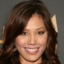
\includegraphics[scale=1.8]{celeba_orig28.png}} 
\hspace{0.5cm}
\subfigure[pic2, Original]{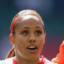
\includegraphics[scale=1.8]{celeba_orig6.png}}
\hspace{0.5cm}
\subfigure[pic3, Original]{
\includegraphics[scale=1.8]{celeba_orig29.png}}
\hspace{0.5cm}
\subfigure[pic1, generiert]{
\includegraphics[scale=1.8]{celeba_gen28.png}} 
\hspace{0.5cm}
\subfigure[pic2, generiert]{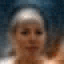
\includegraphics[scale=1.8]{celeba_gen6.png}}
\hspace{0.5cm}
\subfigure[pic3, generiert]{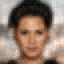
\includegraphics[scale=1.8]{celeba_gen29.png}}
\caption{AutoEncoder für CelebA mit least squares und 48 Channels}
\end{figure}

\bigskip
\uline{Montag, 24.07.17:}
\begin{itemize}
\item Erzeugung gemittelter Bilder, d.h. im Bottleneck der CelebA AutoEncoders zwei (oder mehr) Bilder gemittelt und als ein Bild zurückgeneriert
\begin{itemize}
\item nach wie vor verschwommene Bilder, aber je nach gewählter Kombination der Eingabebilder sind aus jedem Bild einzelne Details gut erkennbar
\end{itemize}

\begin{figure}[H]
\centering
\hspace{0.37cm}
\subfigure[pic1, Original]{
\includegraphics[scale=1.8]{000001.png}} 
\hspace{0.5cm}
\subfigure[gemitteltes Bild]{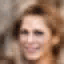
\includegraphics[scale=1.8]{celeba_mean_1_2.png}} 
\hspace{0.5cm}
\subfigure[pic2, Original]{
\includegraphics[scale=1.8]{000002.png}}
\hspace{0.5cm}
\caption{Erzeugung eines gemittelten Bildes aus zwei Originalbildern von CelebA.}
\end{figure}

\item Erzeugung zufälliger Gesichter
\begin{itemize}
\item anfangs nur Rauschen erkennbar
\end{itemize}
\item Verbesserung durch Einbindung einer PCA/ Kovarianzmatrix, sodass Werte (im Bottleneck) mit der entsprechenden Verteilung gesamplet werden können!
\begin{itemize}
\item Danach folgende Bilder:
\end{itemize}

\begin{figure}[H]
\centering
\subfigure{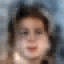
\includegraphics[scale=1.5]{celeba_rand1.png}} 
\hspace{0.5cm}
\subfigure{
\includegraphics[scale=1.5]{celeba_rand2.png}} 
\hspace{0.5cm}
\subfigure{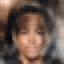
\includegraphics[scale=1.5]{celeba_rand6.png}}
\hspace{0.5cm}
\subfigure{
\includegraphics[scale=1.5]{celeba_rand22.png}}
\hspace{0.5cm}
\subfigure{
\includegraphics[scale=1.5]{celeba_rand43.png}}
\hspace{0.5cm}
\subfigure{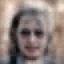
\includegraphics[scale=1.5]{celeba_rand12.png}}
\caption{zufällig erzeugte CelebA-Gesichter}
\end{figure}

\item Einbindung von Schiebereglern, der entlang der Hauptachsen der PCA die Gewichtung der Werte verändert, sodass die zufällig erzeugten Bilder in Echtzeit verändert werden können
\begin{itemize}
\item Veränderungen (bei entsprechend hoher Skalierung der Gewichte) gut erkennbar, jedoch ändern sich bei den meisten Schiebereglern ähnliche \enquote{Eigenschaften} wie Hintergrund, Haarlänge, Haarfarbe... hier muss noch etwas gefeilt werden.
\end{itemize}
\item erstmalige Kombinierung von Generator und Diskriminator, sehr viel Debugging
\end{itemize}

\bigskip
\uline{Dienstag, 25.07.17:}
\begin{itemize}
\item Weitere Bearbeitung der Schieberegler, sodass Bild direkt neben den Schiebereglern angezeigt und aktualisiert wird
\item Debugging des GAN
\end{itemize}

\bigskip
\uline{Mittwoch, 26.07.17:}
\begin{itemize}
\item Debugging des GAN
\begin{itemize}
\item viele Änderungen der loss-Funktionen
\item läuft nun durch, Ergebnisse jedoch noch nicht ausgewertet
\end{itemize}
\end{itemize}

\bigskip
\uline{Donnerstag, 27.07.17:}
\begin{itemize}
\item Verschiedene Versuche, unser GAN zu optimieren und sinnvolle Ergebnisse zu erzielen
\begin{itemize}
\item Abwägung und Balancierung des Trainings des Diskriminators und des Generators. Dabei soll verhindert werden, dass eine Partei gewinnt oder sich beide in einem lokalen Minimum verlieren.
\item Es ist nicht klar, ob sich in unserem Programm noch ein Bug befindet, oder ob es an der Abstimmung der Netzwerke aufeinander hängt. Als Hinweis haben wir bekommen, das nächste Mal die einzelnen Netzwerke nicht selbst zu schreiben, sondern auf funktionierende Netzwerke zurückzugreifen und diese zu kombinieren, um damit die Fehlerquellen einzuschränken.
\item Alternativ noch auszuprobieren: Zusätzlich den AutoEncoder in unser GAN einbauen.
\item Es konnten leider keine guten Ergebnisse erzielt werden! 
\end{itemize}
\end{itemize}


\end{document}
